\documentclass{beamer}
\usepackage{xeCJK}
\setmainfont{ArialMT}
%\setbeamertemplate{frametitle}[default][center]
\setCJKmainfont[BoldFont=Sarasa-Gothic-SC-Bold]{Sarasa-Gothic-SC-Regular}
% 设置中文默认字体
\setCJKsansfont[BoldFont=Sarasa-Mono-SC-Bold]{Sarasa-Mono-SC-Regular}
\mode<presentation> {

\usetheme{default}
%\usetheme{AnnArbor}
%\usetheme{Antibes}
%\usetheme{Bergen}
%\usetheme{Berkeley}
%\usetheme{Berlin}
%\usetheme{Boadilla}
%\usetheme{CambridgeUS}
%\usetheme{Copenhagen}
%\usetheme{Darmstadt}
%\usetheme{Dresden}
%\usetheme{Frankfurt}
%\usetheme{Goettingen}
%\usetheme{Hannover}
%\usetheme{Ilmenau}
%\usetheme{JuanLesPins}
%\usetheme{Luebeck}
%\usetheme{Madrid}
%\usetheme{Malmoe}
%\usetheme{Marburg}
%\usetheme{Montpellier}
%\usetheme{PaloAlto}
%\usetheme{Pittsburgh}
%\usetheme{Rochester}
%\usetheme{Singapore}
%\usetheme{Szeged}
%\usetheme{Warsaw}

%\usecolortheme{albatross}
%\usecolortheme{beaver}
%\usecolortheme{beetle}
%\usecolortheme{crane}
%\usecolortheme{dolphin}
%\usecolortheme{dove}
%\usecolortheme{fly}
%\usecolortheme{lily}
%\usecolortheme{orchid}
%\usecolortheme{rose}
%\usecolortheme{seagull}
%\usecolortheme{seahorse}
%\usecolortheme{whale}
%\usecolortheme{wolverine}
%\usecolortheme{structure}

%\setbeamertemplate{footline} % To remove the footer line in all slides uncomment this line
%\setbeamertemplate{footline}[page number] % To replace the footer line in all slides with a simple slide count uncomment this line

%\setbeamertemplate{navigation symbols}{} % To remove the navigation symbols from the bottom of all slides, uncomment this line
}
\usepackage{fontspec}
\usepackage{bibentry}
\usepackage{graphicx} % Allows including images
\usepackage{booktabs} % Allows the use of \toprule, \midrule and \bottomrule in tables
\usepackage{url}



% 加导航条
%\useoutertheme[width=3\baselineskip,right]{sidebar}
% 目录标数字
\setbeamertemplate{section in toc}[sections numbered] 
% 无序列表用实心点
\setbeamertemplate{itemize item}{\(\bullet \)}
% 设置每页标题格式
% \setbeamertemplate{frametitle}
%   {\vspace{-0.5cm}
%    \insertframetitle
%    \vspace{-0.5cm}}
% 去掉下面没用的导航条
%\setbeamertemplate{navigation symbols}{}
% 设置页脚格式
% \makeatother
% \setbeamertemplate{footline}
% {
%   \leavevmode%
%   \hbox{%
%   \begin{beamercolorbox}[wd=.4\paperwidth,ht=2.25ex,dp=1ex,center]{author in head/foot}%
%     \usebeamerfont{author in head/foot}\insertshortauthor
%   \end{beamercolorbox}

%   \begin{beamercolorbox}[wd=.6\paperwidth,ht=2.25ex,dp=1ex,center]{title in head/foot}%
%     \usebeamerfont{title in head/foot}\insertshorttitle\hspace*{13em}
%     \insertframenumber{} / \inserttotalframenumber\hspace*{0ex}
%   \end{beamercolorbox}}

%   \vskip0pt%
% }
% \makeatletter

% 定义颜色
\definecolor{alizarin}{rgb}{0.82, 0.1, 0.26} % 红色
%\definecolor{DarkFern}{HTML}{407428} % 绿色
%\colorlet{main}{DarkFern!100!white} % 第一种设置方法
\colorlet{main}{red!70!black} % 第二种设置方法
\definecolor{bistre}{rgb}{0.24, 0.17, 0.12} % 黑色
\definecolor{mygrey}{rgb}{0.52, 0.52, 0.51} % 灰色
%\colorlet{main}{green!50!black}
\colorlet{text}{bistre!100!white}

% 不同元素指定不同颜色,fg是本身颜色,bg是背景颜色,!num!改变数值提供渐变色
\setbeamercolor{title}{fg=main}
\setbeamercolor{frametitle}{fg=main}
\setbeamercolor{section in toc}{fg=text}
\setbeamercolor{normal text}{fg=text}
\setbeamercolor{block title}{fg=main,bg=mygrey!14!white}
\setbeamercolor{block body}{fg=black,bg=mygrey!10!white}
%\setbeamercolor{block body}{fg=text}
\setbeamercolor{qed symbol}{fg=main} % 证明结束后的框颜色
\setbeamercolor{math text}{fg=black}
% 设置页脚对应位置颜色
% \setbeamercolor{author in head/foot}{fg=black, bg=mygrey!5!white}
% \setbeamercolor{title in head/foot}{fg=black, bg=mygrey!5!white}
\setbeamercolor{structure}{fg=main, bg=mygrey!10!white} % 设置sidebar颜色

% 左右页间距的排版
% \def\swidth{2.3cm}
% \setbeamersize{sidebar width right=\swidth}
% \setbeamersize{sidebar width left=\swidth}
% \setbeamerfont{title in sidebar}{size=\scriptsize}
% \setbeamerfont{section in sidebar}{size=\tiny}

% \setbeamertemplate{frametitle}
% {\begin{beamercolorbox}[wd=\paperwidth]{frametitle}
%       \strut\hspace{0.5em}\insertframetitle\strut
%       \hfill
%       \raisebox{-2mm}{
\includegraphics[width=1cm]{figures/JI-logo.png}}
%     \end{beamercolorbox}
% }
\setbeamertemplate{bibliography item}[text] %参考文献图标改普通
%----------------------------------------------------------------------------------------
%	TITLE PAGE
%----------------------------------------------------------------------------------------

\title[Exercise Recommendation]{Research on High School Math Exercise Recommendation Based on Graph Neural Network} % The short title appears at the bottom of every slide; the full title is only on the title page

\author{Wangzhihui Mei} % Your name
\institute[UOW] 
{
University of Wollongong \\ % Your institution for the title page
\medskip
\textit{maywzh@gmail.com} % Your email address
}
\date{\today} % Date, can be changed to a custom date

\begin{document}

\begin{frame}
  \titlepage\ % Print the title page as the first slide
\end{frame}

\begin{frame}
  \frametitle{Overview} % Table of contents slide, comment this block out to remove it
  \tableofcontents % Throughout your presentation, if you choose to use \section{} and \subsection{} commands, these will automatically be printed on this slide as an overview of your presentation
\end{frame}

%----------------------------------------------------------------------------------------
%	PRESENTATION SLIDES
%----------------------------------------------------------------------------------------

%------------------------------------------------
\section{Introduction}
%------------------------------------------------
\subsection{Research Background}
\begin{frame}
  \frametitle{Research Background}
  \begin{itemize}
    \item Knowledge State Monitoring
    \item Learning Resource Recommendation
    \item High School Math (Chinese)
  \end{itemize}
\end{frame}

%------------------------------------------------
\subsection{Existing Problems}
\begin{frame}
  \frametitle{Existing Problems}
  \begin{description}
    \item[Inappropriate Recommendation] Exercise recommendation is not based on knowledge mastery
    \item[Disorganized exercise] Labelling knowledge for exercises lacking knowledge tags
    \item[Knowledge evaluation] The difficulty for obtaining knowledge mastery proficiency of the student
    \item[Exercise recommendation] How to recommend appropriate exercises according to their knowledge status
  \end{description}
\end{frame}
%------------------------------------------------
\subsection{Research Cores}
\begin{frame}
  \frametitle{Research Cores}
  \begin{block}{Exercise knowledge labeling}
    A multi-knowledge point labeling algorithm for high school mathematics exercises based on bidirectional LSTM (Bi-LSTM)~\cite{chen2017improving} and graph convolutional neural network (GCN)~\cite{kipf2016semi}.
  \end{block}
  \begin{block}{Knowledge tracing}
    A knowledge tracing model based on Transformer~\cite{vaswani2017attention} architecture with graph attention network embedding.
  \end{block}
  \begin{block}{Exercise recommendation}
    A mathematical exercise recommendation model based on Matching-Ranking~\cite{segev2009context} algorithm.
  \end{block}
\end{frame}
%------------------------------------------------
\section{Proposed Model}
%------------------------------------------------
\subsection{Exercise Knowledge Labelling}
\begin{frame}
  \frametitle{Exercise Knowledge Labelling}
  \framesubtitle{Architecture}
  \begin{figure}
    \centering
    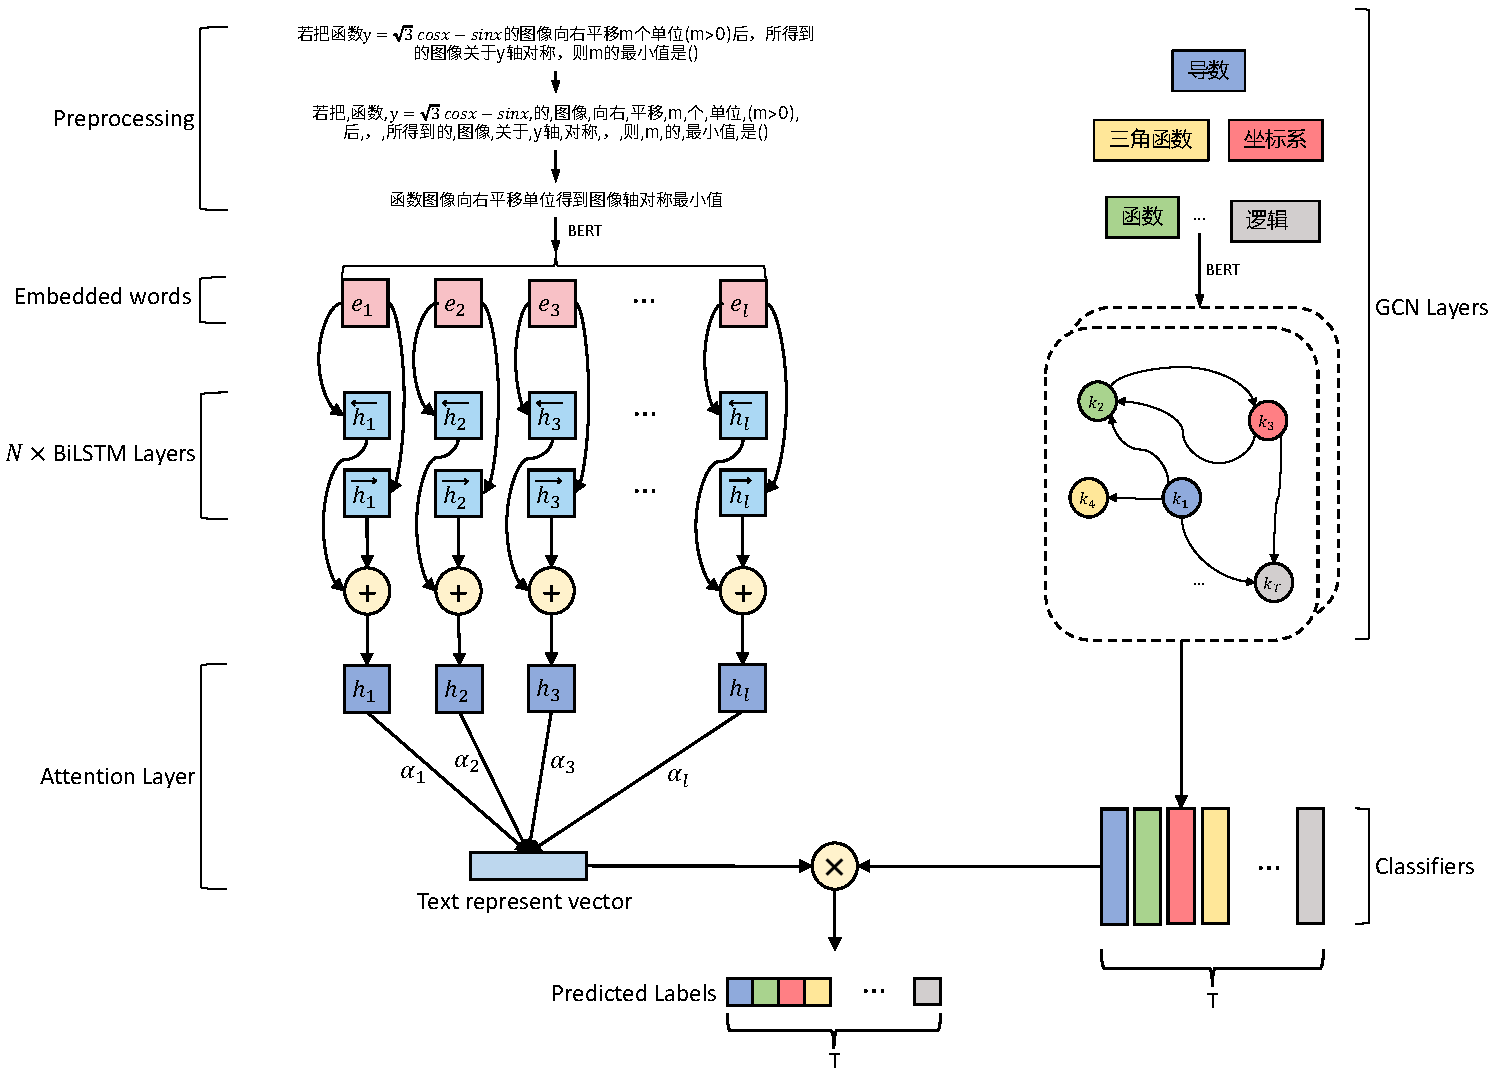
\includegraphics[height=0.80\textheight]{figures/ch2-ov.pdf}
    %\caption{Model architecture}\label{fig:ch2-archi}
  \end{figure}
\end{frame}

%------------------------------------------------
\subsection{Knowledge Tracing}

\begin{frame}
  \frametitle{Knowledge Tracing}
  \framesubtitle{Detail - Knowledge Tracing}
  \begin{figure}
    \centering
    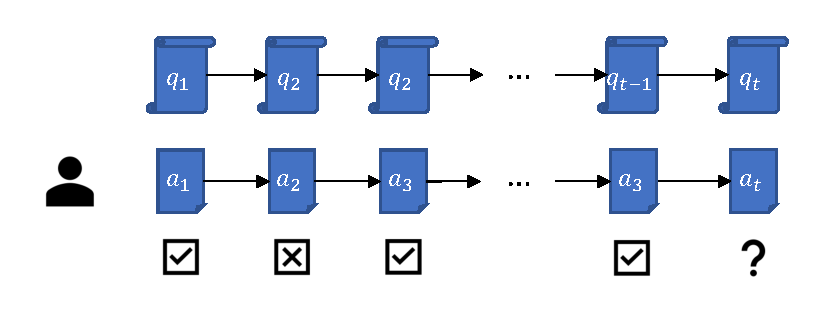
\includegraphics[width=1.0\textwidth]{figures/ch3-model-ktdes.pdf}
    \caption{Knowledge tracing modelling}
  \end{figure}
\end{frame}

\begin{frame}
  \frametitle{Knowledge Tracing}
  \framesubtitle{Detail - Relation Modelling}
  \begin{figure}
    \centering
    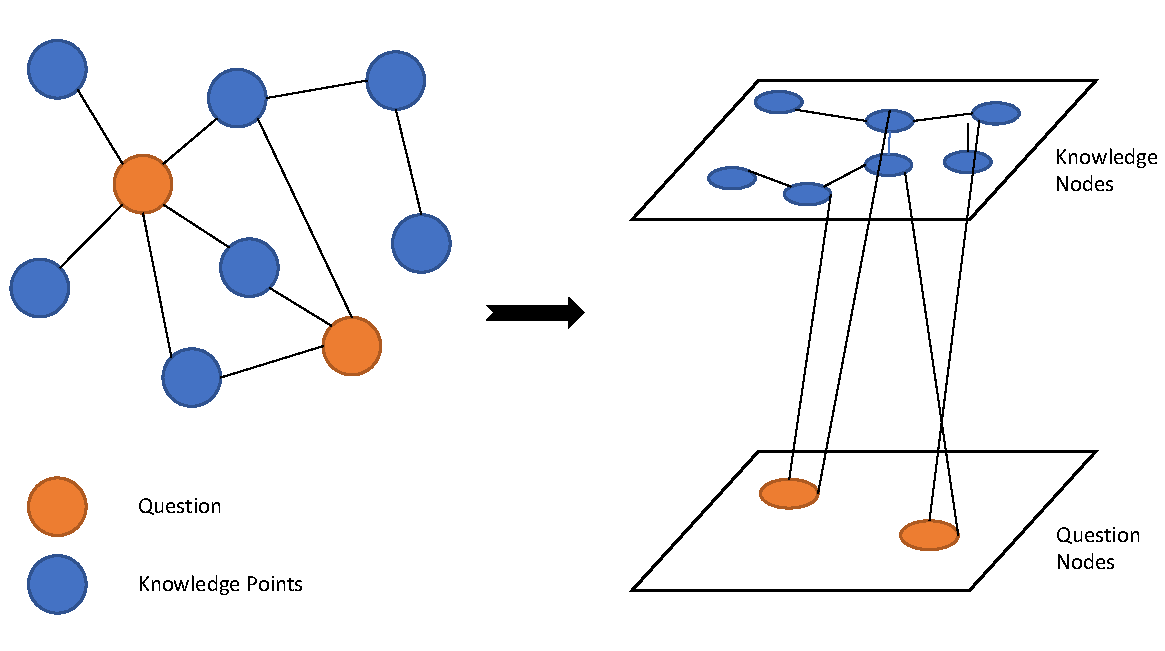
\includegraphics[width=0.94\textwidth]{figures/ch3-gat-kq.pdf}
    \caption{Relation modeling of exercise question and knowledge points}
  \end{figure}
\end{frame}

\begin{frame}
  \frametitle{Knowledge Tracing}
  \framesubtitle{Architecture}
  \begin{figure}
    \centering
    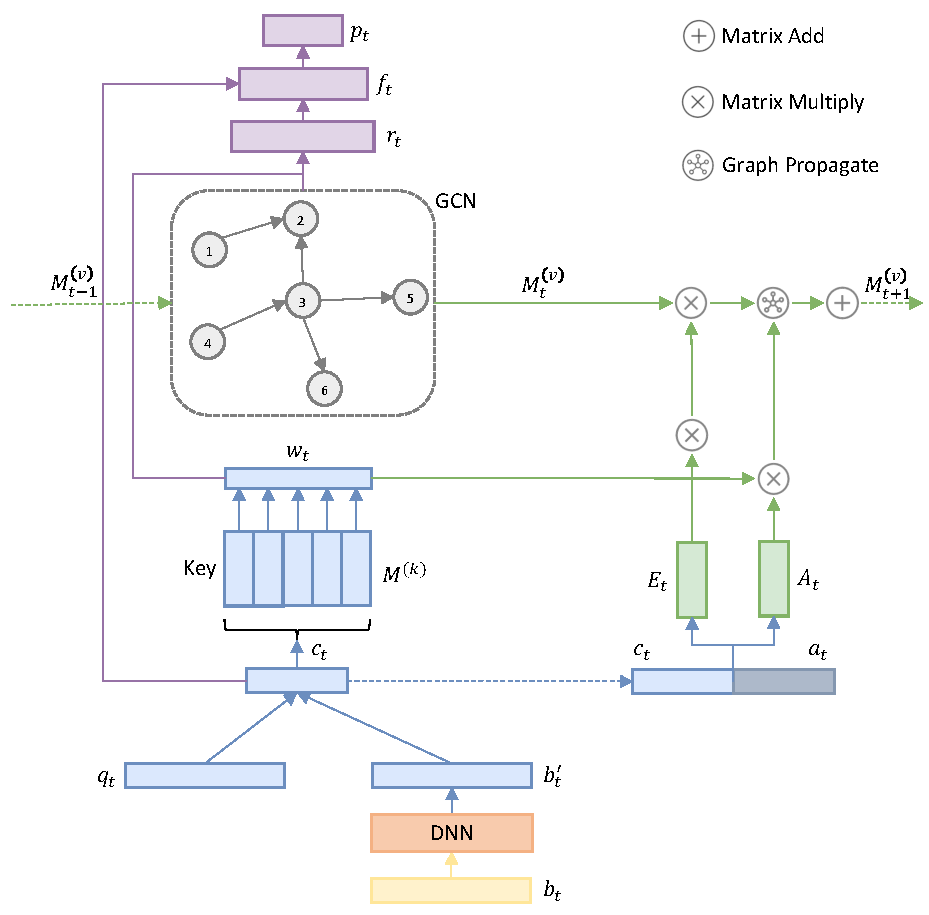
\includegraphics[height=0.80\textheight]{figures/ch3-ov.pdf}
    %\caption{The architecture of proposed knowledge tracing model}
  \end{figure}
\end{frame}



% \begin{frame}
%   \frametitle{Knowledge Tracing}
%   \framesubtitle{Detail}

% \end{frame}


\subsection{Exercise Recommendation}
\begin{frame}
  \frametitle{Exercise Recommendation}
  \framesubtitle{Architecture}
  \begin{figure}
    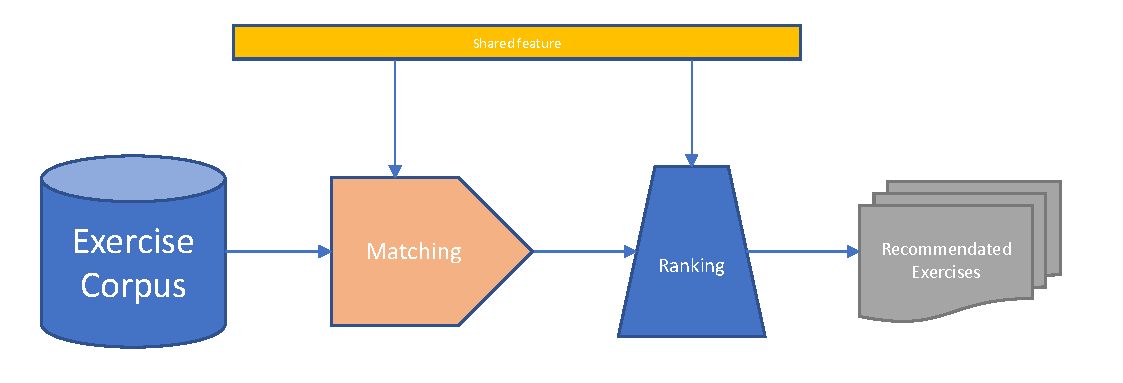
\includegraphics[width=0.9\textwidth]{figures/ch4-ov.pdf}
    \caption{The architecture of recommendation model}
  \end{figure}
\end{frame}

\begin{frame}
  \frametitle{Exercise Recommendation}
  \framesubtitle{Detail - The Matching Phase}
  \begin{figure}
    \centering
    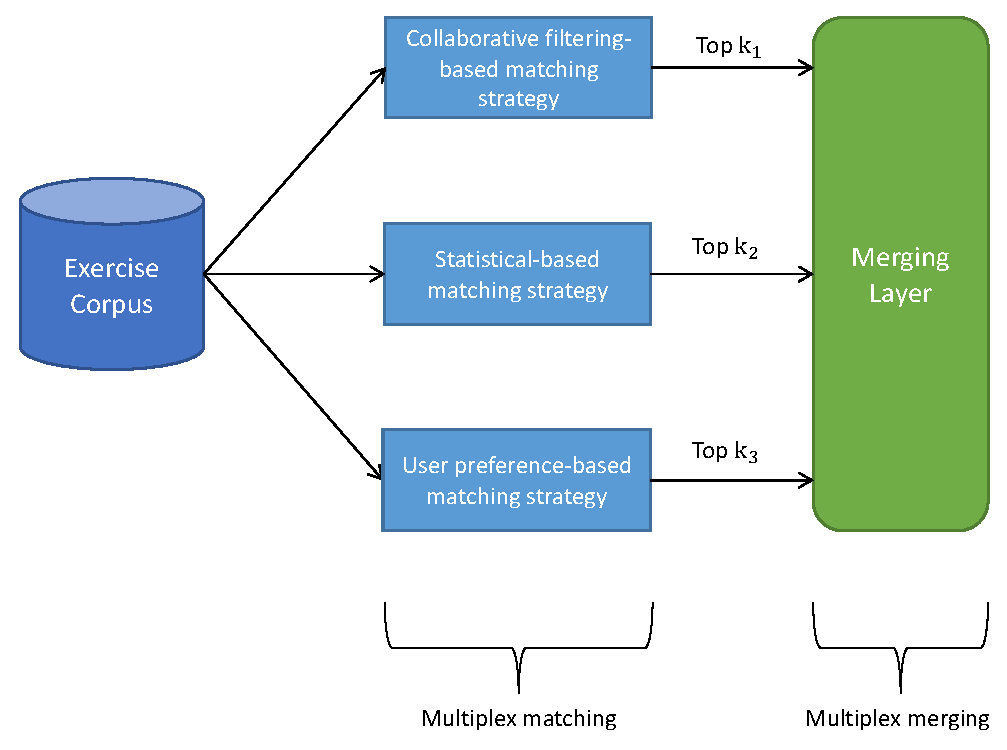
\includegraphics[height=0.7\textheight]{figures/ch4-matching-model.pdf}
    %\caption{The matching phase}
  \end{figure}
\end{frame}

\begin{frame}
  \frametitle{Exercise Recommendation}
  \framesubtitle{Detail - The Ranking Phase}
  \begin{figure}
    \centering
    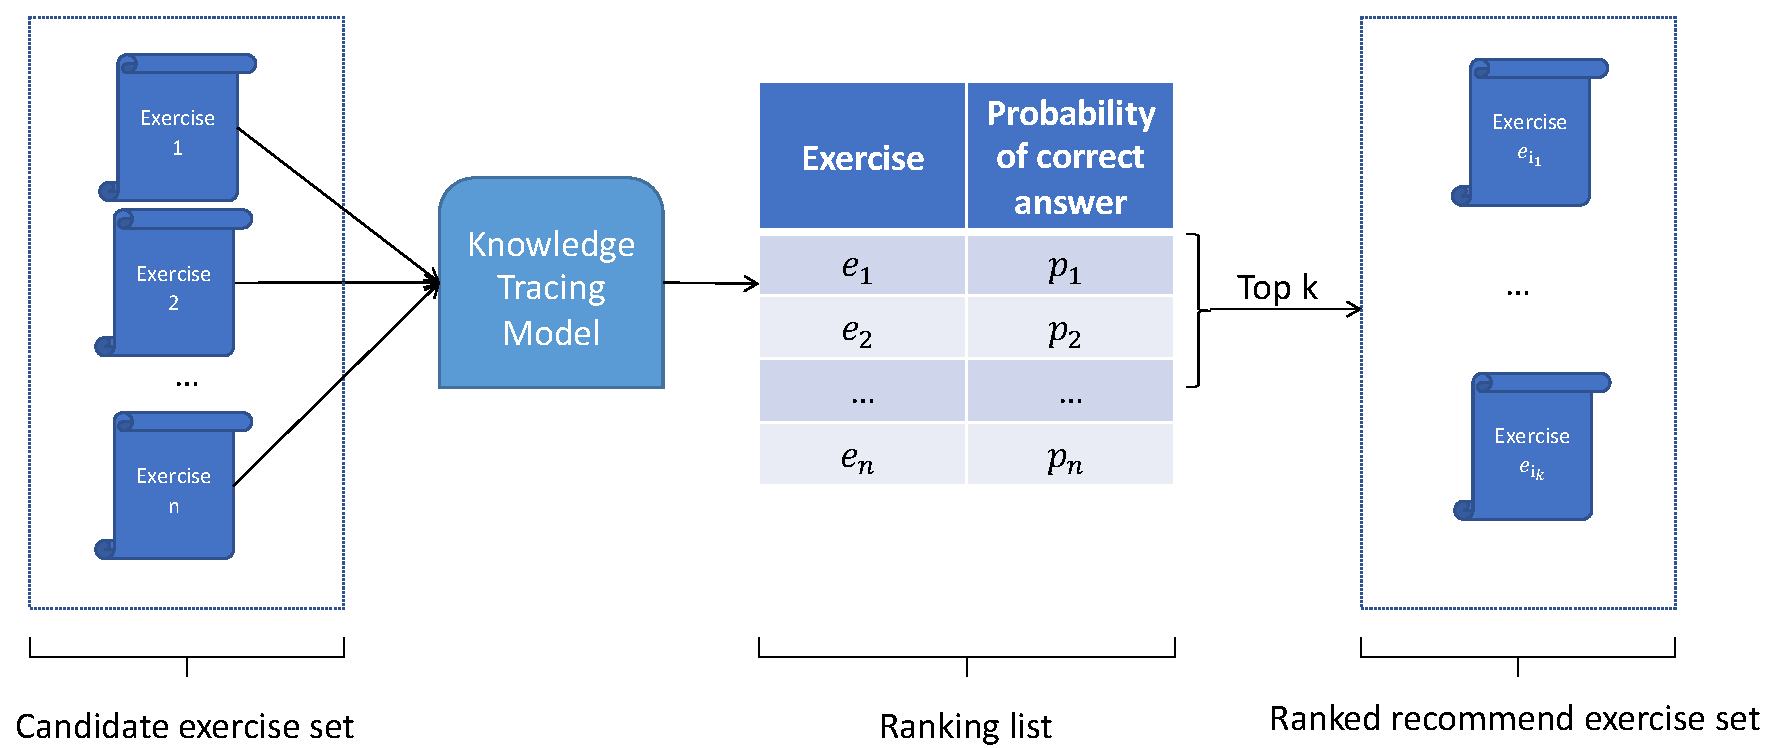
\includegraphics[width=1.0\textwidth]{figures/ch4-ranking-model.pdf}
    %\caption{The ranking phase}
  \end{figure}
\end{frame}

%------------------------------------------------
\section{Experiment Design}
\subsection{Exercise Knowledge Labelling}
\begin{frame}
  \frametitle{Experiment Design}
  \framesubtitle{Exercise Knowledge Labelling}
  \begin{itemize}
    \item Compare with several baseline models
    \item Evaluate the multi-label classification performance
  \end{itemize}
\end{frame}

\begin{frame}
  \frametitle{Experiment Design}
  \framesubtitle{Knowledge Tracing}
  \begin{block}{Basic Method}
    Compare with other KT baseline models BKT~\cite{yudelson2013individualized}、DKT~\cite{piech2015deep}、DKVMN~\cite{chen2017improving} and GKT~\cite{nakagawa2019graph}
  \end{block}
  \begin{table}[htbp!]
    \centering
    \caption{Dataset Statistics}\label{tbl:ch2-tb1}
    \scalebox{0.7}{
      \begin{tabular}{ccccc}
        \toprule
        Dataset   & \#students & \#exercises & \#knowledge points & \#interactions \\
        \midrule
        ASSIST15  & 19,917     & 102,396     & 100                & 709K           \\
        ASSIST17  & 1,709      & 4,117       & 102                & 943K           \\
        STATICS11 & 333        & 1,223       & 156                & 189K           \\
        \bottomrule
      \end{tabular}}
  \end{table}
\end{frame}

\begin{frame}
  \frametitle{Experiment Design}
  \framesubtitle{Exercise Recommendation}
  \begin{itemize}
    \item Compared with conventional Collaborative Filtering and Random Recommendation
    \item Using adapted KT dataset for testing
    \item Check if the selected exercise is in the final recommendation list
  \end{itemize}
\end{frame}


\section{Result and Analysis}
\begin{frame}
  \frametitle{Result}
  \framesubtitle{Exercise Knowledge Labeling}
  \begin{table}[htbp!]
    \caption{The performance comparison between baseline and proposed knowledge labelling models.}\label{tbl:ch2-result-bsline1}
    \centering
    \begin{tabular}{ccccc}
      \toprule
      Metrics           & \(\operatorname{F1}_{macro}\) & \(\operatorname{F1}_{micro}\) & \(\operatorname{Acc}_{ML}\) & \(\operatorname{F1}_{ML}\) \\
      \midrule
      BiLSTM+Attention  & 0.824                         & 0.924                         & 0.874                       & 0.926                      \\
      fastText          & 0.846                         & 0.922                         & 0.854                       & 0.916                      \\
      TextCNN           & 0.761                         & 0.923                         & 0.857                       & 0.917                      \\
      \textbf{Proposed} & \textbf{0.912}                & \textbf{0.932}                & \textbf{0.888}              & \textbf{0.937}             \\
      \bottomrule
    \end{tabular}
  \end{table}
\end{frame}

\begin{frame}
  \frametitle{Result}
  \framesubtitle{Exercise Knowledge Labeling}
  \begin{table}[htbp!]
    \caption{The multi-label classification performance of proposed model.}\label{tbl:ch2-result-detail}
    \centering
    \begin{tabular}{ccccc}
      \toprule
      Class          & Precision & Recall & F1 Score & Support \\
      \midrule
      三角函数       & 0.957     & 0.710  & 0.815    & 31      \\
      函数奇偶性     & 0.946     & 0.930  & 0.938    & 187     \\
      导数           & 0.918     & 0.866  & 0.892    & 247     \\
      平面向量       & 0.942     & 0.961  & 0.951    & 204     \\
      数列           & 0.996     & 0.971  & 0.983    & 243     \\
      逻辑与命题关系 & 0.958     & 0.883  & 0.919    & 180     \\
      集合           & 0.907     & 0.867  & 0.886    & 45      \\
      \midrule
      Micro avg      & 0.951     & 0.915  & 0.932    & 1137    \\
      Macro avg      & 0.946     & 0.884  & 0.912    & 1137    \\
      Weighted avg   & 0.951     & 0.915  & 0.932    & 1137    \\
      Samples avg    & 0.951     & 0.935  & 0.937    & 1137    \\
      \bottomrule
    \end{tabular}
  \end{table}
\end{frame}


\begin{frame}
  \frametitle{Result}
  \framesubtitle{Knowledge Tracing}
  \begin{table}[htb]
    \centering
    \caption{The performance comparison between baseline and proposed knowledge tracing models.}\label{tbl:ch3-performance}
    \begin{tabular}{cccc}
      \toprule
      Model    & ACC (\%)                    & AUC (\%)                   & Training time (sec) \\
      \midrule
      DKT      & \(76.99\pm 0.08 \)          & \(81.79\pm 0.09\)          & \(2,731\)           \\
      DKVMN    & \(75.63\pm 0.19 \)          & \(79.58\pm 0.27\)          & \(3,378\)           \\
      NPA      & \(77.09\pm 0.08\)           & \(81.81\pm 0.13\)          & \(3,872\)           \\
      SAKT     & \(76.37\pm 0.15\)           & \(80.77\pm 0.09\)          & \(4,367\)           \\
      \midrule
      Proposed & \(\mathbf{81.34\pm 0.25} \) & \(\mathbf{83.20\pm 0.25}\) & \(4,597\)           \\
      \bottomrule
    \end{tabular}
  \end{table}
\end{frame}

\begin{frame}
  \frametitle{Result and Analysis}
  \framesubtitle{Exercise Recommendation}
  \begin{table}[htb]
    \caption{The performance comparison between baseline and proposed recommendation models.}\label{tbl:ch4-exp-result}
    \centering
    \setlength{\tabcolsep}{7mm}{
      \begin{tabular}{cc c }
        \toprule
        Model    & ACC             & AUC             \\
        \midrule
        CF       & 0.6329          & 0.6627          \\
        DKT      & 0.7741          & 0.7906          \\
        \midrule
        Proposed & \textbf{0.7997} & \textbf{0.7923} \\
        \bottomrule
      \end{tabular}}
  \end{table}
\end{frame}


\section{Conclusion}
\begin{frame}
  \frametitle{Conclusion}
  \begin{itemize}
    \item The three modules of the proposed model satisfy the requirements of the design
    \item The proposed model achieves better performance compared with baseline models.
  \end{itemize}
\end{frame}
%------------------------------------------------

\begin{frame}[allowframebreaks]{References}
  \bibliographystyle{plain}
  %\bibliographystyle{amsalpha}
  %\bibliography{mybeamer} also works
  \bibliography{./ref.bib}
\end{frame}

%------------------------------------------------

\begin{frame}
  \Huge{\centerline{The End}}
\end{frame}

%----------------------------------------------------------------------------------------

\end{document}